\section{Firefox OS}
\label{sec:firefoxOS}

\subsection{Overview}

As said before
Firefox OS is the open-source operating system targeting mobile devices being
developed by Mozilla and based on Web technologies \cite{MozillaFirefoxOS}.
All the apps in Firefox OS
are Web pages since they are built using only Web technologies and, except when
some special Javascript API are required, can run in a Web browser.
To create an app from a previous Web page you only need a manifest
file that stores some metadata about the app and an image to use as icon. The
files
\href{http://fred-wang.github.io/MathUI2014/demos/app/manifest.webapp}{demos/app/manifest.webapp}
and
\href{http://fred-wang.github.io/MathUI2014/demos/app/icon.png}{demos/app/icon.png},
respectively a manifest and a icon,
show the extra files needed to create an app for
\href{http://fred-wang.github.io/MathUI2014/demos/app/index.html}{demos/app/index.html}.

Although the Web was initially created to share knowledge, today it is also used
as a platform to create knowledge (e.g. Wikipedia) and in a near future
significant part of the content created on the Web will be done using mobile
devices. For science, technology, engineering and mathematics there is a lack of
tools to deal with math that need to be addressed by a ``Math Suite''.

In the next section we give more details about the ``Math Suite'' and
after that we present some of the demos written by Mozilla MathML community.

\subsection{Math Suite}

Like an office suite is a collection of softwares intended to be used by
knowledge workers an Math Suite is a collection of softwares intended to be used
by someone who makes intensive use of math. The basic components of an Math
Suite is a text processor with math support and a symbolic math programming
language, like Mathematica, but the suite could also have:
\begin{itemize}
  \item search engines for math expressions;
  \item WYSIWYG math editor;
  \item markup converters (e.g. LaTeX to MathML and MathML to LaTeX);
  \item handwriting recognition;
  \item 2D drawing tool that helps with, for example,
    \href{http://fred-wang.github.io/MathUI2014/demos/2-mathml-in-svg.svg}{demos/2-mathml-in-svg.svg};
  \item 3D drawing tool that helps with, for example,
    \href{http://fred-wang.github.io/MathUI2014/demos/6-mathml-in-webgl.html}{demos/6-mathml-in-webgl.html};
  \item scripting tool that helps with, for example,
    \href{http://fred-wang.github.io/MathUI2014/demos/3-mathml-javascript.html}{demos/3-mathml-javascript.html};
  \item accessibility to users with disabilities;
  \item Copy \& Paste
  \item and more.
\end{itemize}

Many of the applications, whether or not it is part of the Math Suite,
share a set of functions. For
example the search engine can be used by a text processor and by an ebook
reader. Having
these functions available in an open source Javascript library will make easy to
develop new Web applications that can be customized into standalone applications
to run in desktop and mobile devices.

\begin{figure}[!htb]
  \centering
  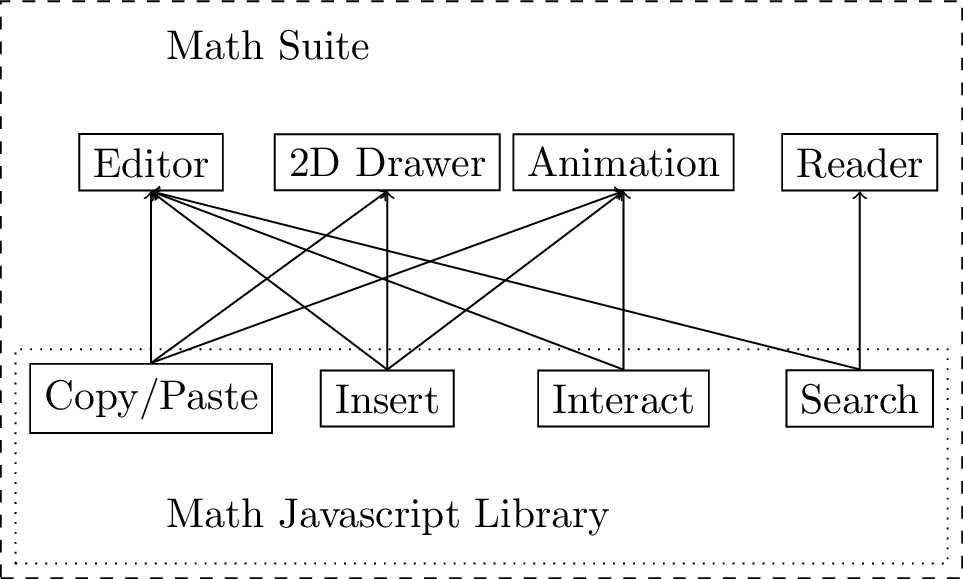
\includegraphics[width=.5\textwidth]{math-suite-diagram.png} \\
  Figure: Illustration of Math Suite.
\end{figure}

The authors of this work started writing this Javascript library as small
independent libraries as well as some demos that use them.

\subsection{Math Cheat Sheet}

This is a basic app with a collection of common K-12 equations available at
\href{http://r-gaia-cs.github.io/math-cheat-sheet/}{http://r-gaia-cs.github.io/math-cheat-sheet/}.
The equations are organized in sections and a table of contents is provided to
help jumping from one section to another.

Although it is a basic app, a LaTeX to MathML conversion was necessary
(we used TeXZilla, see section \ref{sec:texzilla})
 and it is a nice way to show that Firefox OS supports
MathML. At the moment, only the unstable version of Firefox OS supports copy
and paste. However, one can run this app in Firefox Desktop with the MathML Copy
add-on installed and verify that it is possible to
copy and paste the MathML and LaTeX representation of the equations.

Other nice features that can be added to this app in the future include:
\begin{itemize}
  \item link to resource like Wikipedia related to the equation,
  \item search bar to quickly find the desired equation,
  \item customization of equations, \ldots
\end{itemize}

\subsection{TeXZilla App}
\label{sec:texzillapp}

This is a note-taking app for math available at
\href{http://r-gaia-cs.github.io/TeXZilla-webapp/}{http://r-gaia-cs.github.io/TeXZilla-webapp/}.
It takes as input LaTeX expression, shows a preview of it refreshed during
input and enables the user to save it.

The conversion from LaTeX to MathML is performed by TeXZilla
(see section \ref{sec:texzilla})
and no internet connection is required. The save functionality
uses IndexedDB, ``an API for client-side storage of significant amounts of
structured data and for high performance searches on this data using indexes''
as explained at Mozilla Developer Network, there is a W3C Candidate
Recommendation.

This app also has some buttons to help the user to enter LaTeX commands like
{\tt \textbackslash frac} and {\tt \textbackslash sqrt}. Right now the buttons
only cover a few commands since the best solution is for the mobile devices
to have a virtual keyboard for math (we have plans to integrate
such keyboard into Firefox OS) and desktop users can rely on a similar keyboard
made available as an add-on.

\subsection{DynAlgebra}

This is a Dynamic Algebra \cite{Nicaud1}, ``algebraic calculations
on a computer by direct manipulation'', app available at
\href{http://r-gaia-cs.github.io/DynAlgebra/}{http://r-gaia-cs.github.io/DynAlgebra/}.
The idea of Dynamic Algebra is about twenty years old and could help
students to learn formula structure and transformations and help every users to
produce step by step calculations. However, most of the previous implementations
have not been successful.

The last known implementation of Dynamic Algebra was done in EpsilonWriter
\cite{Nicaud2} as a Java application and covers:
\begin{description}
  \item[internal drag \& drop] like convert $x + y + z$ into $y + x + z$,
  \item[external drag \& drop] as dropping a formula on another formula,
  \item[on click calculation] like convert $x + x$ into $2 x$ and
  \item[rewriting rules] like convert $x^{-n}$ into $\frac{1}{x^n}$.
\end{description}

Our app, written in Javascript, is really still at a prototype level compared
to EpsilonWriter and only partially
covers the ``on click calculation''. However, it uses MathML as storage format
and that enables it to work in documents not intended to be used for Dynamic Algebra.

For input of equations our app uses TeXZilla since we do not have a WYSIWYG
editor yet.
